% !TEX root = main.tex

\section{Testing Architectures}
\label{sec:archs}

We experimented with three types of network architectures, which we call "Inception Net", "Res Net", "Andreas Net". 
Each of these networks are inspired by previous work, but were adapted by us to fit our task. 
For each architecture we will describe their structure, the normalization techniques we applied and the results. 
 
For normalization techniques we applied $L_{1}$ regularization on the fully connected layers, batch normalization on the convolutional layer, and dropout. 
For Inception Net and Res Net, our activation function is the Rectified Linear Unit (ReLu), $f(x) = \max(0, x)$. 
For Andreas Net, our activation function is the Leaky Rectified Linear Unit, $f(x) = \max(a, ax)$ where $a$ is referred to as the slope. 
We obtain all of our outputs using the soft-max function over 2 units. 
We predict the class with higher probability, giving us a binary output. 

For each network, we experimented with various normalization constants, network hyper-parameters (i.e. pool size), slopes, etc. 
Within this paper we report only on the best combination of parameters. 

For each network we plot the accuracy and loss across epochs for the training and validation set and report the final accuracy on the test set. 
We also, for most networks, show the confusion matrix.
For all of the following results we used 50,000 data points (split into 80\%/10\%/10\% for training, validation and testing) from our balanced data set. 

Overall, none of these networks were able to achieve an accuracy rate higher then our re-implemented GQ-CNN. 
We can rank the networks from worst to best by accuracy: Res Net, Inception Net, Andreas Net. 

\subsection{Inception Net}

\begin{figure}[t!]
    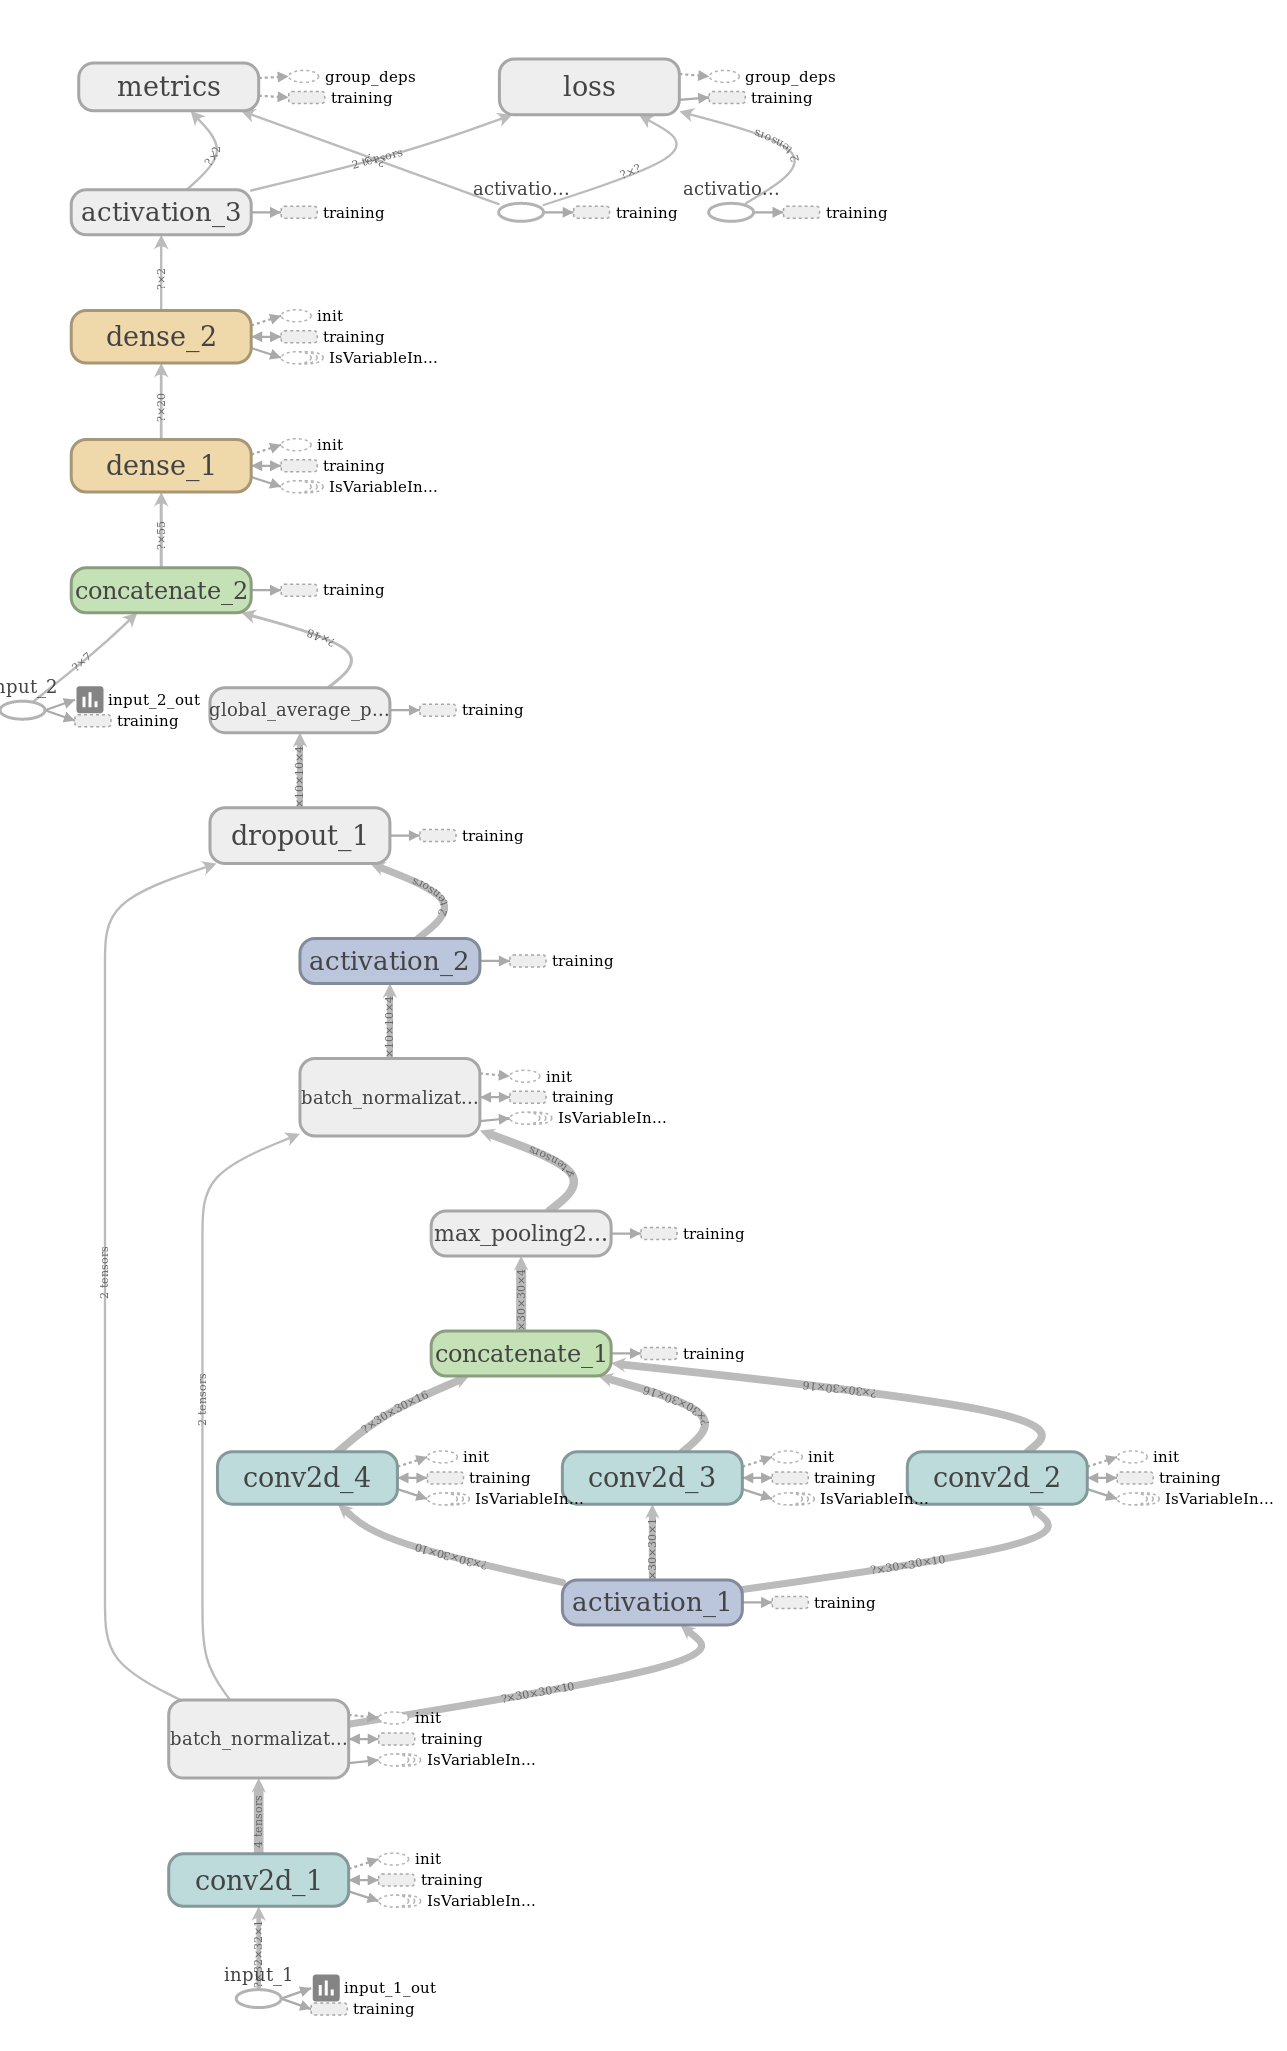
\includegraphics[width=0.99\columnwidth]{figs/inception_net.png}
\caption{Inception Net Architecture. We provide the following labels: Convolution (Conv), Batch Normalization (BN), ReLU (Rectifer Linear Unit), Concatenate (Concat), Dropout (Drop), Global Average Pooling (GAP), Fully Connected (FC), SoftMax (SM).} \label{fig:inception_net}
\end{figure}

\begin{figure*}[t!]
    \centering
    \begin{subfigure}[t]{0.32\textwidth}
        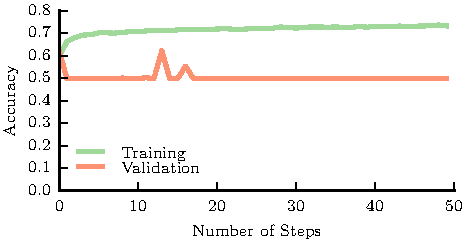
\includegraphics[width=0.9\columnwidth]{figs/inception_accuracy.pdf}
        \caption{Accuracy of Inception Net} \label{fig:accuracy}
        \end{subfigure}
    \begin{subfigure}[t]{0.32\textwidth}
        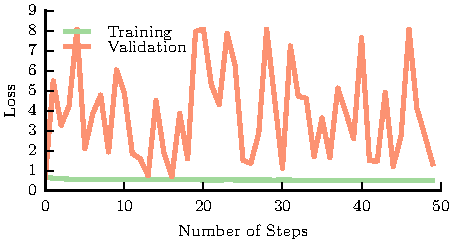
\includegraphics[width=0.9\columnwidth]{figs/inception_loss.pdf}
        \caption{Loss of Inception Net} \label{fig:loss_inception}
    \end{subfigure}
		\begin{subfigure}[t]{0.32\textwidth}
        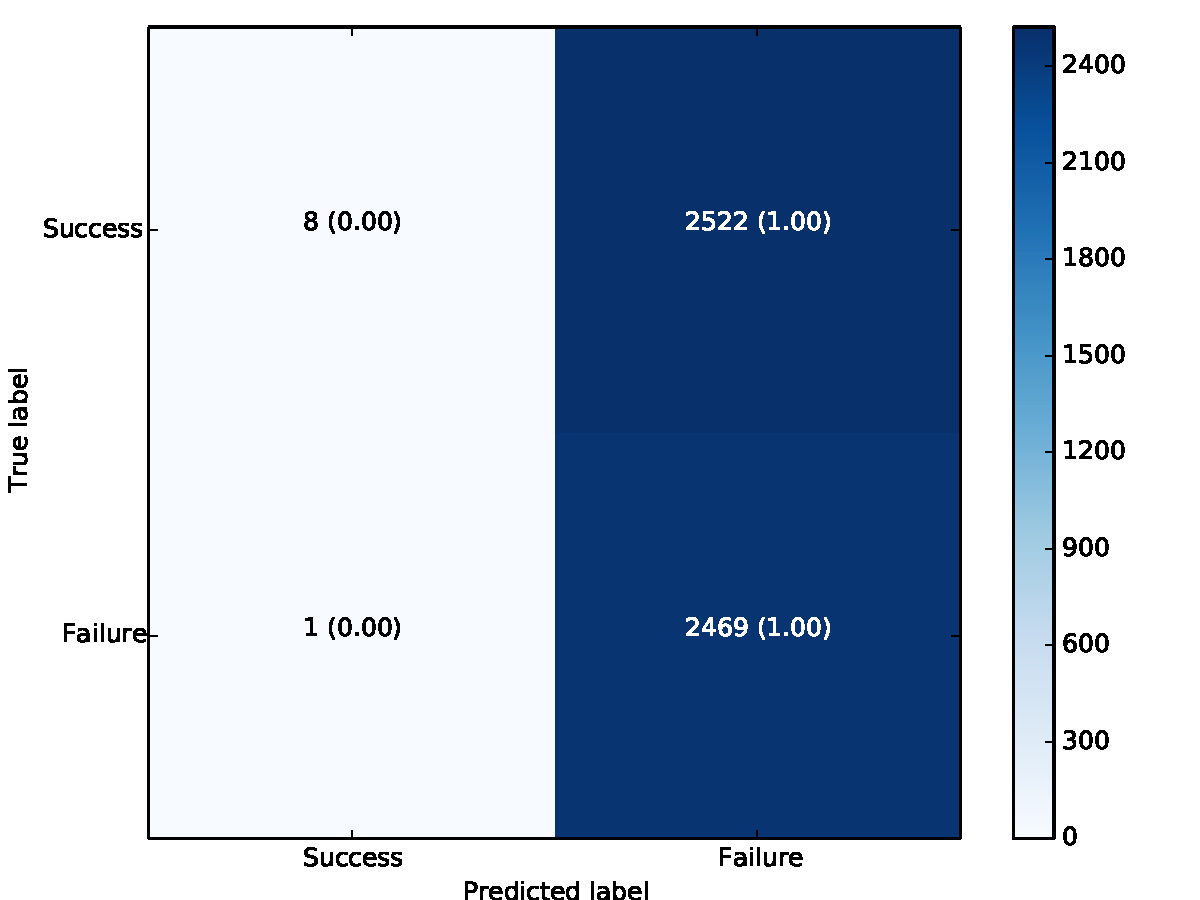
\includegraphics[width=0.8\columnwidth]{figs/confusion_inception.pdf}
        \caption{Confusion Matrix} \label{fig:confusion_inception}
    \end{subfigure}
\caption{We plot the accuracy rate and loss of the Inception Net over training epochs for the training and validation set. This network seems to overfit based off of the difference between the accuracy of the training and validation sets. Our confusion matrix in the rightmost column shows we over predicted failure.} \label{fig:inceptionnet_results}
\end{figure*}

The first network architecture we will explore is the Inception Network~\cite{szegedy2015going}, visualized in \figref{fig:inception_net}. 
This network style was originally designed to increase the depth and width of a network while keeping computational load the same while operating on ImageNet~\cite{deng2009imagenet}. 

The inception network begins with 1 convolution layer in the beginning with 10 filters of size 3x3. 
We apply batch normalization to the output of this layer at ReLU as the activation function. 
We then pass that to three parallel convolutional layers of sizes 1x1, 3x3, and 5x5, each with 16 filters. 
These outputs are concatenated on the depth dimension and passed through a max pooling layer of size 3x3 and stride 1x1.
We apply batch normalization, ReLu activation and a dropout of 70\%. 
The outputs are flattened with global average pooling and then the $z$ value is concatenated on. 
We then pass through two fully connected units of size 25 and 2 respectively.  
We apply the softmax function to these final two units to obtain our output for binary classification.

Our accuracy and loss are shown in \figref{fig:inceptionnet_results}. 
While our training accuracy quickly reaches 70\%, our validation accuracy only rarely spikes above nominal 50\%. 
This poor learning is reflected in the plot of our loss function (\figref{fig:loss_inception}) for our validation set, which never stabilizes. 
Our final accuracy on our training set was 50\%, which, is unimpressive given a binary classification task on a balanced data set. 
Looking at our confusion matrix in \figref{fig:confusion_inception}, our network almost always predicted failure. 
While from a robotic execution perspective this means we are unlikely to execute a failure-likely grasp, the over-prediction of failure also means we are unlikely to execute any grasp. 

For tuning this network, we tried using a larger number of filters at each step, testing with 64, 32 and 20 filters. 
However, the initial loss of the network was very high, and it would not decrease substantially or at all during training. Likewise, max pooling of 2x2 was tested, however this did not bring any benefits to the training either. 
An extra inception "layer" was added after the dropout, however this also resulted in unusually high losses. 
It is worth noting that because dimensions of our data is small, it was not feasible to add many layers. 
We selected a high dropout rate in order to let the network "learn" which of the mappings learned better features and thus was not modified during the experiments. 
As for the $z$ input, a fully connected layer of 16 units was tried, but it did not have much effect on our validation accuracy. 


\subsection{Res Net}

\begin{figure}[t!]
    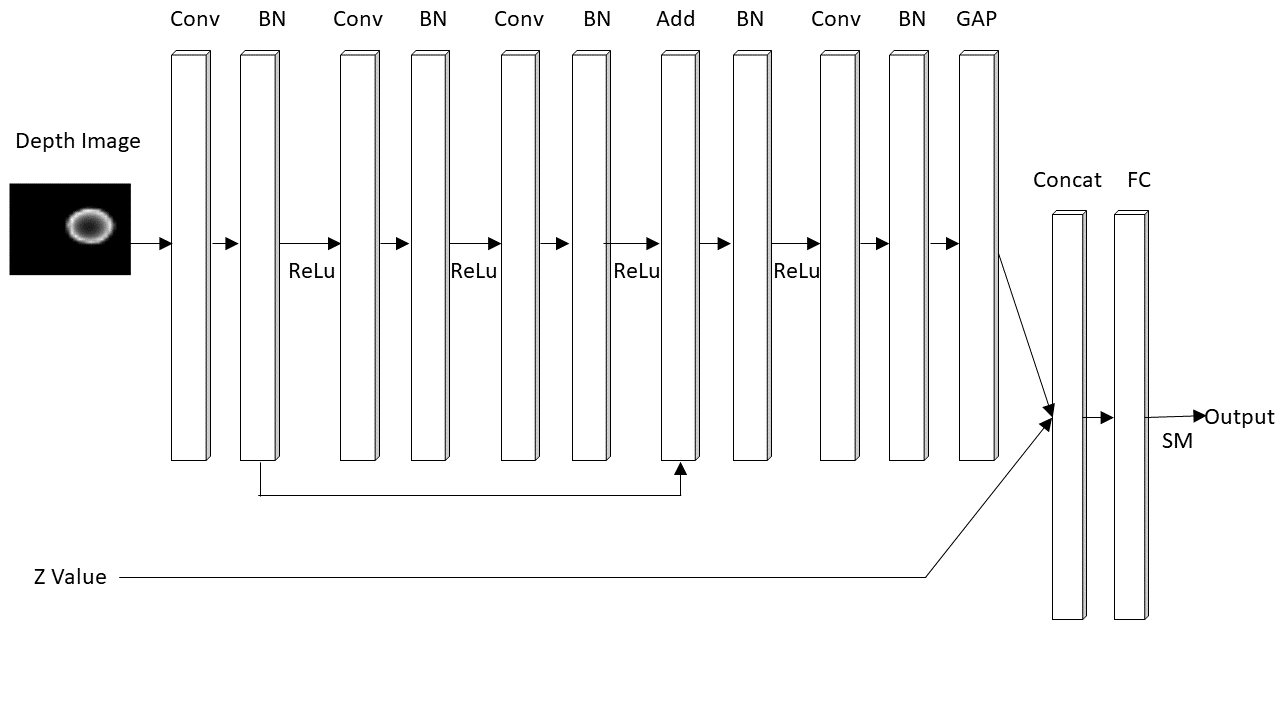
\includegraphics[width=0.99\columnwidth]{figs/res_net.png}
\caption{Res-Net Architecture. We provide the following labels: Convolution (Conv), Batch Normalization (BN), ReLU (Rectifer Linear Unit), Add (Add), Global Average Pooling (GAP), Fully Connected (FC), SoftMax (SM).} \label{fig:res_net}
\end{figure}

Our residual network (called "Res Net" in this discussion) is visualized in \figref{fig:res_net}. 
It consists of one convolutional layer, with 16 filters of size 3x3.
We then apply batch normalization and ReLu as an activation function.
At this point, the output of this layer branches, such that this same output is passed through two more convolution layers of 8 filters 7x7 and 32 filters 3x3used as dimension reduction. 
After each of those two convolution layers is a layer of batch normalization and activation by ReLu.
The output of these two layers is added to their input and then passed through batch normalization and activation by ReLu.
This is then passed to another convolution layer of 8 filters of 1x1 for further dimension reduction. 
We then apply batch normalization and ReLu activation once more before flattened with global average pooling. 

Like for the other network, the $z$ value is concatenated to this output before passing it to a classifier with a fully connected layer of 2 hidden units.
We obtain our output via the softmax function.

Our accuracy and loss are shown in \figref{fig:resnet_results}. 
Our training accuracy nears 80\% and our validation accuracy varies between 50\% and 70\%, depending on when we stop our network. 
This stopping criteria is reflected in our loss graph, which also fluctuates for our validation set. 
Doing slightly worse then Inception Net, our final test accuracy is 48\%. 
Looking at our confusion matrix, our learning algorithm over predicted success, in stark contrast to our Inception Net. 
In practice, given the large quantity of false positives, our robot would execute many grasps that are likely to fail, wasting time and resources. 

For tuning this network, we also tried increasing the number of filters to 64 and 30, and the kernel sizes where permuted (switched around layers). 
However, the model did not do any better or worse than the set of hyper-parameters described above. 
While we experimented with adding a convolution layer to the identity path in the Res Net of 32 filters and kernel size of 5x5, this was not successful since the network never escaped from the 50\% accuracy. 
We also tried using $L_{1}$ regularization on the fully connected layers in the reported architecture. 
However this increased significantly the initial loss and it did not help with the final validation accuracy.

\begin{figure*}[t!]
    \centering
    \begin{subfigure}[t]{0.32\textwidth}
        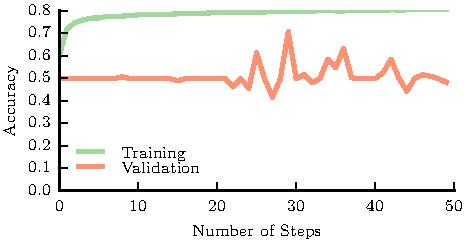
\includegraphics[width=0.9\columnwidth]{figs/res_net_accuracy.pdf}
        \caption{Accuracy} \label{fig:accuracy_res}
        \end{subfigure}
    \begin{subfigure}[t]{0.32\textwidth}
        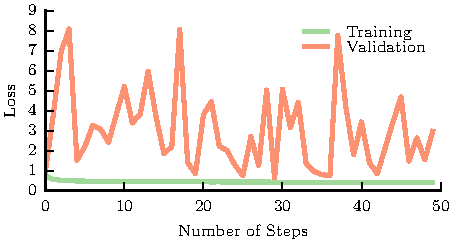
\includegraphics[width=0.9\columnwidth]{figs/res_net_loss.pdf}
        \caption{Loss} \label{fig:loss_res}
    \end{subfigure}
		\begin{subfigure}[t]{0.32\textwidth}
        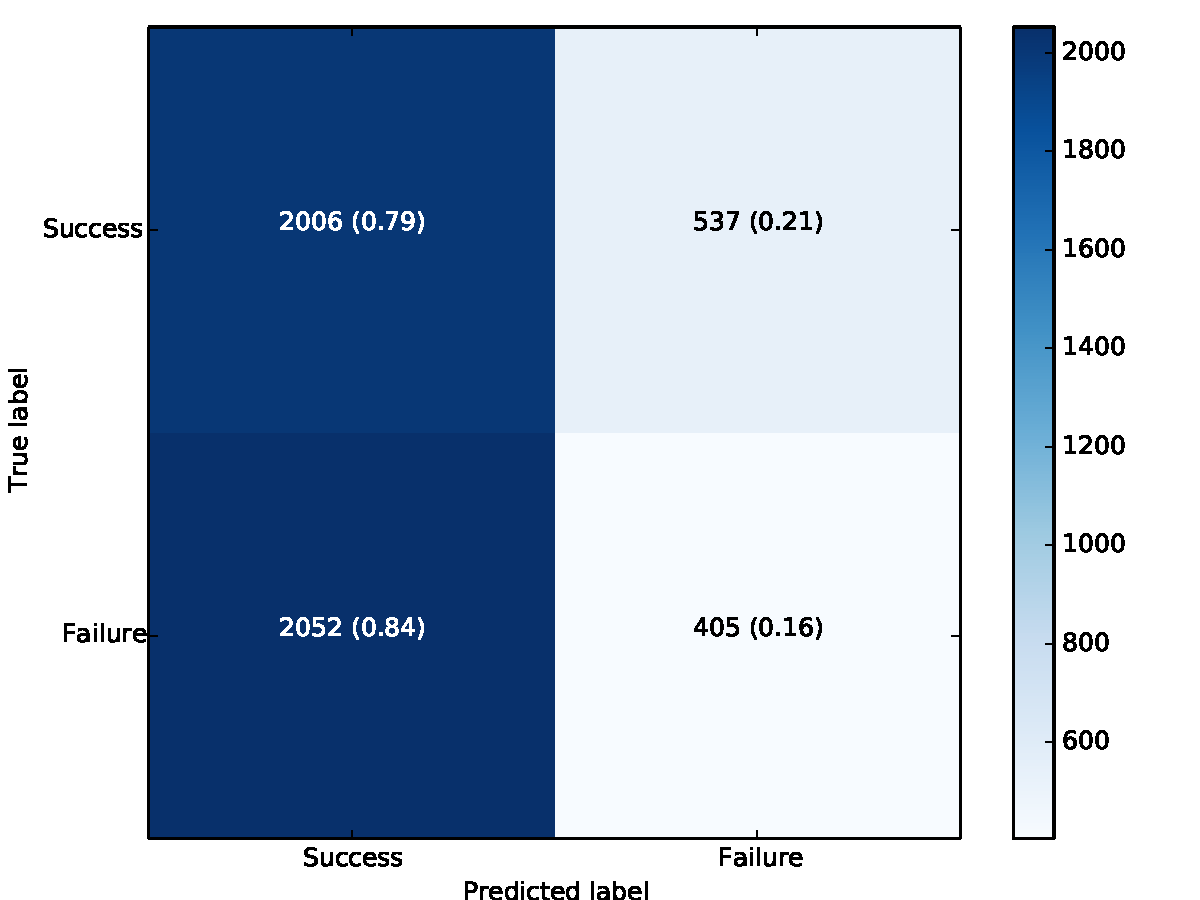
\includegraphics[width=0.8\columnwidth]{figs/confusion_resnet.pdf}
        \caption{Confusion Matrix} \label{fig:confusion_res}
    \end{subfigure}
\caption{We plot the accuracy rate and loss of the Res Net over training epochs for the training and validation set. There is still overfitting in this network, there is odd oscillation of the validation accuracy. Our confusion matrix in the rightmost column shows we over predicted success.} \label{fig:resnet_results}
\end{figure*}

\subsection{Andreas Net}

\begin{figure}[t!]
    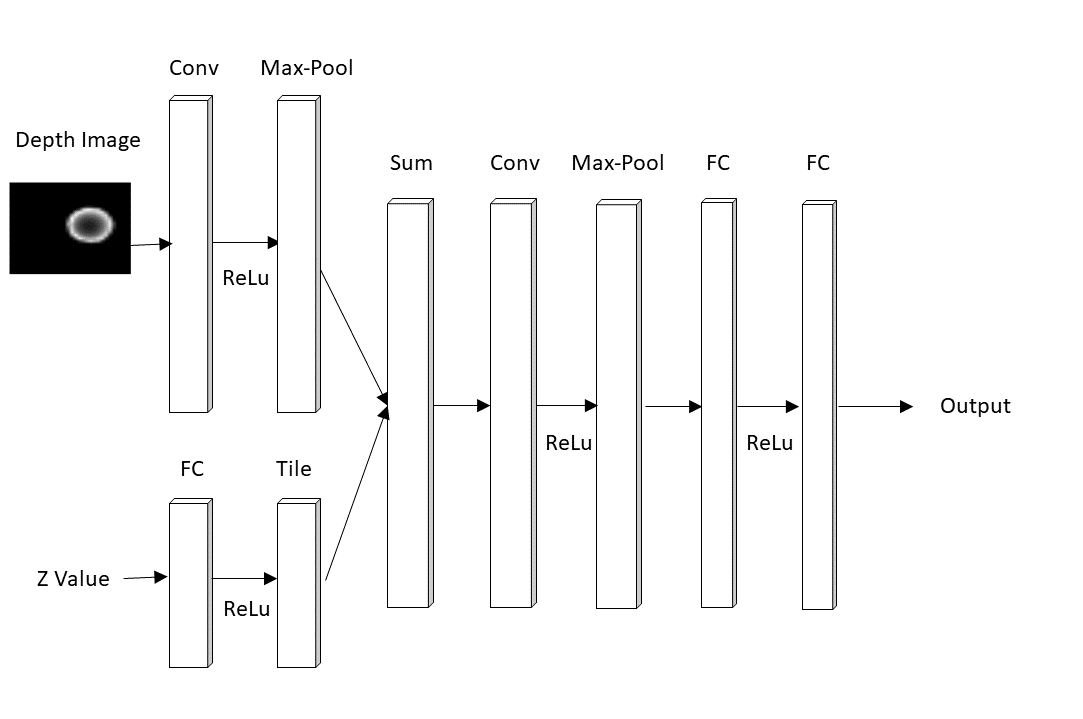
\includegraphics[width=0.99\columnwidth]{figs/andreas_net.png}
\caption{Andreas Net Architecture. We provide the following labels: Convolution (Conv), Leaky Rectified Linear Unit (LR), Max-Pooling (Max-Pool),  Fully Connected (FC), Tiling (Tile), Sum (Sum), Fully Connected (FC), SoftMax (SM).} \label{fig:andreas_net}
\end{figure}

The last architecture we consider is from~\cite{viereck2017learning} and will be referred to as "Andreas Net". 
It is visualized in \figref{fig:andreas_net}. 
The network, like GQ-CNN, was designed for robotics grasping and uses depth images as input. 
However, \cite{viereck2017learning} creates a closed-loop controller that guides the gripper to the object to be grasped. 
Thus their CNN learns the distance to the nearest grasp function used by the controller. 
Despite its original use as a regression network, we adapt it to our classification task. 

The depth image is passed through one convolutional layer, with 20 filters of size 5x5. 
This output is activated by a Leaky ReLu with slope 0.3 before a batch normalization layer. 
We pass this to a max-pooling layer of size 2x2 and stride 1x1. 
The z-value is passed through a full connected layer of 20 units with $L_{1}$ regularization of $\lambda=0.1$.
We pass this through Leaky ReLu, again with slope 0.3, and then tile the output~\cite{ngiam2010tiled}.
The tile operation consists of taking the 1-D vector of 20 elements and, for each scalar, a 14x14 "feature map" is formed by repeating this scalar. 
The output is 20 14x14 "feature maps" are added channel-wise to each of the outputs of one of the convolutional layers.
The outputs of each of these, the processed depth image and processed z-value, are summed.

This result is passed through convolutional layer with 50 filter of size 5x5, followed by Leaky ReLu, with slope 0.3. 
We then apply dropout at rate 0.6 and then a max-pooling layer with size 2x2 and stride 1x1. 
We flatten this output and pass it through a fully connected layer of 20 units and $L_{1}$ regularization with $\lambda = 0.1$. 
This is activated by Leaky ReLU (again slope 0.3) and finally connected to a fully connected layer with 2 hidden units (again with $L_{1}$ regularization at $\lambda=0.1$). 
We apply softmax to these two units to generate our output. 

Our accuracy and loss are shown in \figref{fig:andreas_results}. 
After 30 training steps, our training and validation accuracy improve with our training accuracy near 70\% and our validation wavering between 50\% and 70\%, depending on when we stop training. 
For both networks our loss over time shows little variance. 
Our final test accuracy is 56\%, an improvement over Inception Net and Res Net, but still slightly worse then our re-trained version of the GQ-CNN. 

In developing the network, we first tried the original "Andreas Net" (i.e described in ~\cite{viereck2017learning}), without dropout. 
This did not perform better than random classification. 
However, the introduction of the dropout increased the the final test accuracy to 56\%. 
We also replaced the Leaky ReLU functions with normal ReLU functions, but this decreased the accuracy back to 50\%. 
An additional layer of 50 filters and kernel size of 5x5 was added before the flattening operation, therefore essentially reducing the feature maps to 1x1.  
This did not lead to good generalization. 

As an alternative to the flatten operation, a global average pooling operation was tested instead. 
While this operation has been successfully used in other object detection networks, it did not seem to add much to our network and thus we continued to use the flatten operation. 
For the $L_{1}$ regularization factor, in addition to 0.1 we also tried 0.01 and 0.3, to see whether decreasing or increasing the regularization would affect the final accuracy. 
However, even when changing slightly this factor, we saw high initial loss even after 50 epochs and the network performance was quite poor. 


\begin{figure*}[t!]
    \centering
    \begin{subfigure}[t]{0.49\textwidth}
        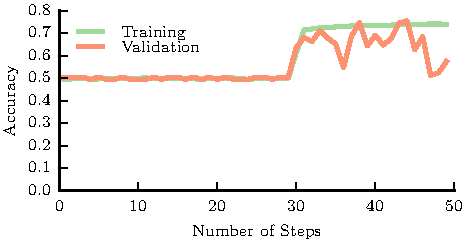
\includegraphics[width=0.9\columnwidth]{figs/andreas_accuracy.pdf}
        \caption{Accuracy} \label{fig:accuracy}
        \end{subfigure}
    \begin{subfigure}[t]{0.49\textwidth}
        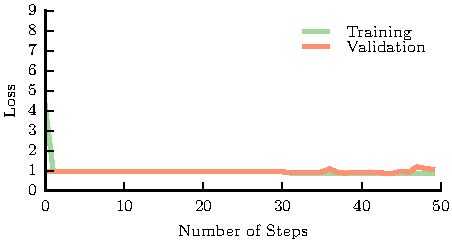
\includegraphics[width=0.9\columnwidth]{figs/andreas_loss.pdf}
        \caption{Loss} \label{fig:loss}
    \end{subfigure}
\caption{We plot the accuracy rate and loss of the Andreas Net over training epochs for the training and validation set. Of our new networks this performs the best, although its validation accuracy also oscillates.} \label{fig:andreas_results}
\end{figure*}